\section{Introduction}        
%%问题背景
\subsection{Problem Background}%%二级章节标题
Asian giant hornets have unexpectedly emerged at Vancouver in September 2019. While humans are not the intended prey of these giant hornets, their stings are extremely painful, often medically complicated, and annually result in several dozen deaths in their Asian home range \parencite{1RSSL}. Moreover, they are also natural enemies of bees and threaten the local honey production. After their first appearance, there have been many mixed sightings of Asian giant hornets in Washington State as a neighboring area, which caused public anxiety.

Some sightings were determined to be Asian giant hornets, but many other sighted insects proved not to be them. So the state must decide how to prioritize the use of limited resources for further follow-up investigations based on the sighting reports provided by witnesses.

Therefore, it is necessary to interpret the data provided by the public report, prioritize it according to the possibility, and design a sysytem to solve the problem of government agency resource allocation.

%%问题重述
\subsection{Restatement and Analysis}
In this problem, the materials given are 4440 sighting reports and related documents on Asian giant hornets (in the following we will call them pests). The reports include sighting photos, detection date, and information processed by the US Department of Agriculture. We are required to carry out statistical modeling to solve the prioritization of sighting reports and propose solution to related issues.

We should only use these materials to explore and solve the following aspects:
\begin{itemize}%2/5完成，2/8需要改进%已改进
    \item Establish a predictive model to forecast the spread of this pest over time, and improve the accuracy of the region as much as possible, which will pave the foundation for subsequent models.
    \item Create a model that evaluates the similarities between other types of insects and pest, analyze the influencing factors and discuss the output results to predict the possibility of misclassification.
    \item Prioritize sighting reports based on our judgment indices and models, so that reports with higher priority are more likely to be positive sightings.
    \item Solve how to update the model and the frequency of updating when the report data is expanded.
    \item Determine an index to show the eradication of pests.
\end{itemize}

We have analyzed the requirements and issues raised, and believe that it is necessary to apply an evaluation system to build a model for ranking all witness reports. This model includes sub-models such as the prediction of pest transmission and evaluation of the similarity between other insects and pests.

%%工作介绍，简明叙述解题方法和主要成果
\subsection{Our work}
Our work follows the following workflow, as shown in the Figure \ref{fig:workflow}.
\begin{figure}[H]
    \centering
    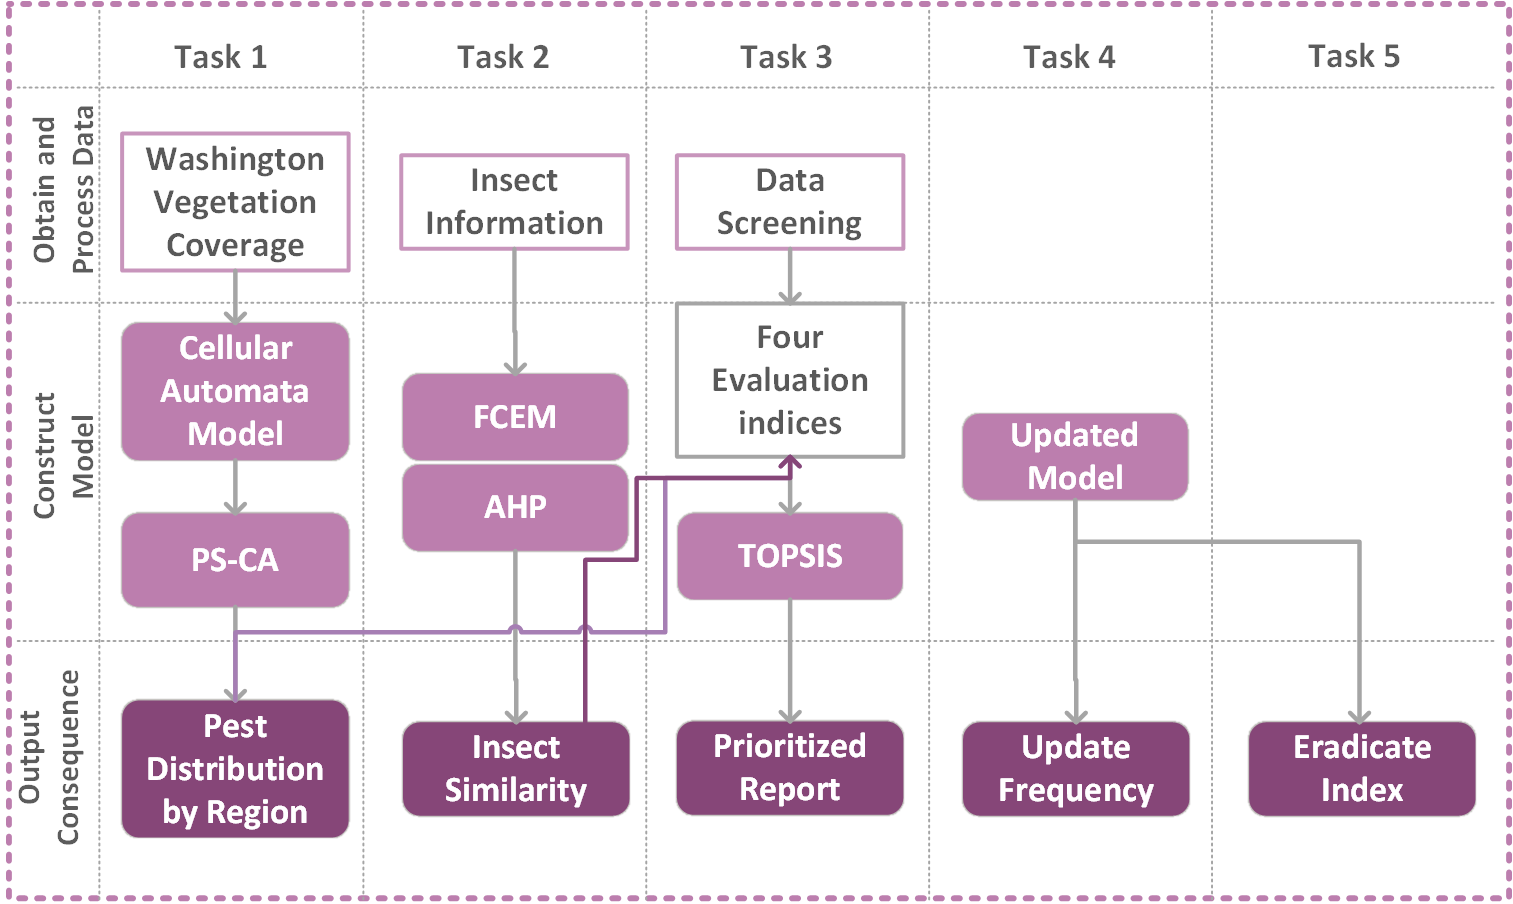
\includegraphics[scale = 0.45]{Chapter-2021C/images-2021C/workflow.png}
    \caption{Our Workflow.}
    \label{fig:workflow}
\end{figure}
\begin{itemize}                %%以圆点方式给出各点
    \item In task 1, we fully understand the reproduction characteristics and living habits of pests, consider the geographical factors of Washington State, decide to apply cellular automata to simulate the distribution of pests over time, and visualize the results on the map. Finally, we further test the model and analyze that the accuracy of the model is a $150m \times 150m$ area.
    \item For task 2, we try to build a similarity database according to the similarity of other types of insects and pest  from a visual perspective. In the paper, we select nine other types of insects and compare their characteristics to pest based on FCEM in terms of size, abdomen, head, chest, and nest. Then we use AHP to analyze the weight of each feature. Finally, the possibility of nine types of insects being misclassified is discussed from the visual similarity.
    \item As to task 3, we first use LR to filter the report to remove invalid reports with little information. Then we determine four indices to measure the accuracy of the report and use TOPSIS to score each report to obtain the ranking results. The four indices are the probability of occurrence, time activeness, note effectiveness and possibility of misclassification.
    \item As for task 4, we make efforts to optimize our model and clarify the update frequency. Starting from the perspective of multi-point invasion of pest, the new accurate sighting location is set as a new starting point in the PS-CA model, While destroy of pest nest is set as clearing an existing point. From the perspective of human intervention to prevent and control pests, we adjust the growth curve of pest every year to achieve reasonable simulation results.
    \item In terms of task 5, we set an index for the degree of eradication based on the optimized model. Then we run the PS-CA model to calculate the intervention period until the degree satisfy the criteria. In addition, we also conduct a sensitivity analysis of the model and achieve ideal results.
\end{itemize}